%=============================================================
%  TEMPLATE PRESENTATION BEAMER - KHOA HTTT - UIT
%  Dành cho sinh viên báo cáo môn học & khóa luận
%=============================================================
\documentclass[10pt,aspectratio=169]{beamer}
\usepackage[utf8]{vietnam}
\usepackage{amsmath,amssymb,amsfonts}
\usepackage{booktabs,array,longtable}
\usepackage{graphicx}
\usepackage{tikz}
\usetikzlibrary{shapes,arrows,arrows.meta,positioning,calc,
                shapes.geometric,fit,decorations.pathreplacing,
                decorations.markings,backgrounds,shadows}
\usepackage{pgfplots}
\pgfplotsset{compat=1.18}
\usepackage[many]{tcolorbox}
\usepackage{fontawesome5}
\usepackage{hyperref}
\usepackage{listings}
\graphicspath{{figures/}}

%=============================================================
%  1. TEMPLATE CUSTOMIZATION (Màu sắc, Logo và Thông tin)
%  Sinh viên thay đổi các thông số dưới đây để tùy biến slide
%=============================================================
\definecolor{uitblue}{RGB}{108,79,59}       % Màu chủ đạo (Nâu đậm của header/bìa)
\definecolor{uitdark}{RGB}{74,53,37}        % Màu phụ (Nâu tối ở dải bìa/footer)
\definecolor{accent}{RGB}{197,140,50}       % Màu nhấn mạnh (Vàng Gold)
\definecolor{accentlt}{RGB}{222,178,110}    % Màu nhấn phụ (Vàng cát)
\definecolor{greenteal}{RGB}{100,120,80}    % Màu ví dụ/thực hành (Sage Green)
\definecolor{lightgray}{RGB}{248,245,240}   % Màu nền ấm của slide (Cream/Ivory)
\definecolor{textgray}{RGB}{60,55,50}       % Màu chữ thân (Charcoal)

\newcommand{\titlebgimage}{../../report/slides/title_bg.png}
\newcommand{\sectionbgimage}{../../report/slides/section_bg.png} % Tên tệp ảnh nền trang ngăn cách section (nếu có)     % Tên tệp ảnh nền mờ trang bìa (nếu có)
\newcommand{\logonhomNC}{../../report/slides/logo_nhom_nc.png}   % Logo nhóm nghiên cứu/Lab (nếu có)
\newcommand{\logonhomthuchien}{../../report/slides/logo_nhom_thuchien.png} % Logo nhóm thực hiện/CLB (nếu có)
\newcommand{\gvhd}{[]}         % Giáo viên hướng dẫn (nếu có)
\newcommand{\slidewatermark}{../../report/slides/logo_nhom_nc.png} % Tệp ảnh mờ làm hình nền từng slide (để trống nếu không dùng)
\newcommand{\contactemail}{ftisu@uit.edu.vn} % Email liên hệ hiển thị ở trang bìa

%=============================================================
%  2. THÔNG TIN BÁO CÁO (Metadata)
%=============================================================
\title[Nutrition5k + TiMePReSt]{Ước lượng dinh dưỡng từ ảnh RGB-D (Nutrition5k) với huấn luyện song song kiểu pipeline TiMePReSt}
\subtitle{Báo cáo tiến độ nghiên cứu (14/10 -- 17/10/2026)}
\author{Người thực hiện: [An Văn Kết]}
\date{Ngày báo cáo: 17/10/2026}

%=============================================================
%  3. BEAMER THEME OVERRIDE (Cấu hình hiển thị - KHÔNG NÊN SỬA)
%=============================================================
\usetheme{default}
\usecolortheme{default}
\setbeamertemplate{navigation symbols}{}

% Thiết lập màu sắc các thành phần Beamer
\setbeamercolor{palette primary}{bg=uitblue,fg=white}
\setbeamercolor{frametitle}{bg=uitblue,fg=white}
\setbeamercolor{title}{bg=uitblue,fg=white}
\setbeamercolor{author in head/foot}{bg=uitdark,fg=white}
\setbeamercolor{title in head/foot}{bg=uitblue,fg=white}
\setbeamercolor{date in head/foot}{bg=uitdark!80,fg=white}
\setbeamercolor{section in head/foot}{bg=uitblue!70,fg=white}

\setbeamercolor{block title}{bg=uitblue!18,fg=uitdark}
\setbeamercolor{block body}{bg=uitblue!5,fg=textgray}
\setbeamercolor{alertblock title}{bg=accent!20,fg=accent!80!black}
\setbeamercolor{alertblock body}{bg=accent!5,fg=textgray}
\setbeamercolor{exampleblock title}{bg=greenteal!20,fg=greenteal!70!black}
\setbeamercolor{exampleblock body}{bg=greenteal!5,fg=textgray}
\setbeamercolor{item}{fg=uitblue}
\setbeamercolor{subitem}{fg=accent}
\setbeamercolor{enumerate item}{fg=uitblue}
\setbeamercolor{normal text}{fg=textgray}
\setbeamercolor{structure}{fg=uitblue}

% Định dạng tiêu đề slide (Frametitle)
% Thiết lập hình nền mờ dưới từng slide (Watermark)
\usebackgroundtemplate{
  \ifx\slidewatermark\empty\else
    \expandafter\IfFileExists\expandafter{\slidewatermark}{
      \begin{tikzpicture}[remember picture, overlay]
        \node[opacity=0.03, anchor=center] at (current page.center) {
          \includegraphics[width=0.3\paperwidth]{\slidewatermark}
        };
      \end{tikzpicture}
    }{}
  \fi
}

\setbeamertemplate{frametitle}{
  \vskip2pt
  \begin{beamercolorbox}[wd=\paperwidth,ht=0.56cm,dp=0.2cm,leftskip=0.4cm]{frametitle}
    \usebeamerfont{frametitle}\insertframetitle
    \ifx\insertframesubtitle\empty\else
      \;{\small\textcolor{accentlt}{$\triangleright$}}\;\usebeamerfont{framesubtitle}\textcolor{accentlt}{\insertframesubtitle}
    \fi
  \end{beamercolorbox}
  \vskip-2pt
  \begin{beamercolorbox}[wd=\paperwidth,ht=1.2pt,dp=0pt]{palette primary}
    \color{accent}\rule{\paperwidth}{1.2pt}
  \end{beamercolorbox}
}

% Định dạng chân trang (Footline)
\setbeamertemplate{footline}{
  \begin{beamercolorbox}[wd=\paperwidth,ht=0.4cm,dp=0.12cm]{author in head/foot}
    \hspace{0.3cm}{\scriptsize\faUniversity\; UIT -- Khoa Hệ thống Thông tin}
    \hfill
    {\scriptsize Báo cáo khoa học}
    \hfill
    {\scriptsize\insertframenumber/\inserttotalframenumber\hspace{0.3cm}}
  \end{beamercolorbox}
}

% Định dạng đầu trang (Headline)
\setbeamertemplate{headline}{
  \begin{beamercolorbox}[wd=\paperwidth,ht=0.06cm]{section in head/foot}
    \color{accent}\rule{\paperwidth}{0.06cm}
  \end{beamercolorbox}
}

% Định dạng ký hiệu danh sách (Itemize bullets)
\setbeamertemplate{itemize item}{\color{uitblue}\faCircle[regular]}
\setbeamertemplate{itemize subitem}{\color{accent}$\triangleright$}
\setbeamertemplate{enumerate item}{\color{uitblue}\insertenumlabel.}

% Định dạng trang bìa (Title Page)
\setbeamertemplate{title page}{
  \begin{tikzpicture}[remember picture, overlay]
    \fill[uitblue] (current page.north west) rectangle ([yshift=-0.58\paperheight]current page.north east);
    \fill[uitdark] ([yshift=-0.58\paperheight]current page.north west)
         rectangle ([yshift=-0.62\paperheight]current page.north east);
    \fill[lightgray] ([yshift=-0.62\paperheight]current page.north west)
         rectangle (current page.south east);
         
    \expandafter\IfFileExists\expandafter{\titlebgimage}{
      \node[opacity=0.10, anchor=center] at (current page.center) {\includegraphics[width=\paperwidth,height=\paperheight]{\titlebgimage}};
    }{}
         
    \node[white, anchor=north west, font=\large\bfseries, align=left, text width=0.9\paperwidth] (univ) at
         ([xshift=0.5cm, yshift=-0.4cm]current page.north west)
         {\faUniversity\quad TRƯỜNG ĐẠI HỌC CÔNG NGHỆ THÔNG TIN -- UIT \\
          \small\normalfont Khoa Hệ thống Thông tin $|$ Nhóm nghiên cứu FTISU};
          
    \node[white, anchor=north west, font=\LARGE\bfseries, text width=0.88\paperwidth, align=left] (title) at
         ([yshift=-0.25cm]univ.south west)
         {\inserttitle};
         
    \node[accentlt, anchor=north west, font=\normalsize\itshape, text width=0.88\paperwidth, align=left] (subtitle) at
         ([yshift=-0.15cm]title.south west)
         {\insertsubtitle};
         
    \node[uitdark, anchor=north west, font=\small, align=left] at
         ([xshift=0.8cm, yshift=-0.66\paperheight]current page.north west)
         {\faUser\quad \insertauthor \\
          \ifx\gvhd\empty\else
            \faGraduationCap\quad GVHD: \gvhd \\
          \fi
          \faEnvelope\quad \contactemail \\
          \faCalendar\quad \insertdate};
         
    % Trang trí dòng kẻ đứng
    \draw[accent,line width=4pt]
         ([xshift=0.5cm,yshift=-0.65\paperheight]current page.north west)
      -- ([xshift=0.5cm,yshift=-0.85\paperheight]current page.north west);

    % Hiển thị Logo nhóm nghiên cứu / câu lạc bộ / khoa ở góc dưới bên phải
        % Hiển thị Logo: Nhóm NC nằm bên TRÁI nhóm thực hiện (Góc dưới bên phải)
    \expandafter\IfFileExists\expandafter{\logonhomthuchien}{
        % Vẽ Logo nhóm thực hiện trước, neo vào góc và đặt tên node là 'logo2'
        \node[anchor=south east, inner sep=0pt] (logo2) at ([xshift=-0.5cm, yshift=0.4cm]current page.south east) {
            \includegraphics[height=0.7cm]{\logonhomthuchien}
        };
        
        \expandafter\IfFileExists\expandafter{\logonhomNC}{
            % Logo nhóm NC sẽ bám vào phía bên TRÁI (west) của logo2
            \node[anchor=east, inner sep=0pt] at ([xshift=-0.2cm]logo2.west) {
                \includegraphics[height=0.7cm]{\logonhomNC}
            };
        }{}
    }{
        % Trường hợp KHÔNG có logo nhóm thực hiện, chỉ có logo nhóm NC
        \expandafter\IfFileExists\expandafter{\logonhomNC}{
            \node[anchor=south east, inner sep=0pt] at ([xshift=-0.5cm, yshift=0.4cm]current page.south east) {
                \includegraphics[height=0.7cm]{\logonhomNC}
            };
        }{}
    }
    \end{tikzpicture}
}

\AtBeginSection[]{
  {
    \usebackgroundtemplate{
      \begin{tikzpicture}[remember picture, overlay]
        \expandafter\IfFileExists\expandafter{\sectionbgimage}{
          \node[anchor=center, inner sep=0pt] at (current page.center) {
            \includegraphics[width=\paperwidth,height=\paperheight]{\sectionbgimage}
          };
        }{}
        \fill[uitblue, opacity=0.92] (current page.north west) rectangle (current page.south east);
      \end{tikzpicture}
    }
    \begin{frame}[plain]
      \centering
      \vspace{1.8cm}
      {\color{white}\Huge\bfseries\thesection}
      \par\vskip 0.3cm
      {\color{accent}\rule{0.5\paperwidth}{2pt}}
      \par\vskip 0.4cm
      {\color{accentlt}\Large\bfseries\insertsectionhead}
    \end{frame}
  }
}

%=============================================================
%  4. CÁC HỘP THÔNG TIN TCOLORBOX
%=============================================================
\tcbuselibrary{skins,breakable}

% Hộp UIT mặc định (Màu xanh chủ đạo/nâu đất)
\newtcolorbox{uitbox}[2][]{
  enhanced,
  colback=uitblue!6, colframe=uitblue, coltitle=white,
  fonttitle=\bfseries\small, title={#2},
  boxrule=0.5pt, arc=4pt, left=4pt, right=4pt, top=3pt, bottom=3pt,
  attach boxed title to top left={yshift=-2mm,xshift=4mm},
  boxed title style={colback=uitblue, arc=3pt, boxrule=0pt},
  #1
}

% Hộp Accent nhấn mạnh (Màu vàng nhấn)
\newtcolorbox{accentbox}[2][]{
  enhanced,
  colback=accent!6, colframe=accent, coltitle=white,
  fonttitle=\bfseries\small, title={#2},
  boxrule=0.5pt, arc=4pt, left=4pt, right=4pt, top=3pt, bottom=3pt,
  attach boxed title to top left={yshift=-2mm,xshift=4mm},
  boxed title style={colback=accent, arc=3pt, boxrule=0pt},
  #1
}

% Hộp ví dụ (Màu xanh lá)
\newtcolorbox{greenbox}[2][]{
  enhanced,
  colback=greenteal!6, colframe=greenteal, coltitle=white,
  fonttitle=\bfseries\small, title={#2},
  boxrule=0.5pt, arc=4pt, left=4pt, right=4pt, top=3pt, bottom=3pt,
  attach boxed title to top left={yshift=-2mm,xshift=4mm},
  boxed title style={colback=greenteal, arc=3pt, boxrule=0pt},
  #1
}

%=============================================================
%  5. CÁC MACRO RÚT GỌN (Tô màu từ khóa)
%=============================================================
\newcommand{\highlight}[1]{\textcolor{accent}{\bfseries #1}}
\newcommand{\kw}[1]{\textcolor{uitblue}{\bfseries #1}}

%=============================================================
%  PHẦN THÂN TÀI LIỆU
%=============================================================
\begin{document}
\newcolumntype{L}[1]{>{\raggedright\arraybackslash}p{#1}}
\newcolumntype{R}[1]{>{\raggedleft\arraybackslash}p{#1}}

%--- Trang bìa ---
{
  \usebackgroundtemplate{}
  \begin{frame}[plain]
    \titlepage
  \end{frame}
}

%--- Bài toán ---
\begin{frame}{Bài toán và mô hình}
\begin{columns}[T]
\column{0.49\textwidth}
\begin{uitbox}{\faBullseye\; Bài toán (nhóm FoodAI xác nhận)}
\scriptsize
Một mô hình, ba việc trên ảnh chụp từ trên xuống của Nutrition5k \cite{thames2021nutrition5k}:
\begin{enumerate}
  \item \kw{Nhận diện} món có những nguyên liệu nào (195 nguyên liệu).
  \item \kw{Hàm lượng:} gram từng nguyên liệu; kcal, khối lượng, chất béo, carb, đạm của cả món.
  \item \kw{Vị trí:} bản đồ calories trên ảnh (học yếu, không có mask).
\end{enumerate}
Huấn luyện bằng pipeline 2 GPU với TiMePReSt \cite{dutta2026timeprest}, so với PipeDream \cite{narayanan2019pipedream}, DDP và 1 GPU.
\end{uitbox}

\column{0.47\textwidth}
\begin{uitbox}{\faProjectDiagram\; Mô hình (18 khối, chia được thành stage)}
\scriptsize
\begin{itemize}
  \item ResNet-50 pretrained ImageNet, conv1 4 kênh (kênh depth khởi tạo bằng trung bình 3 kênh RGB) $\rightarrow$ feature 2048$\times$7$\times$7.
  \item Đầu ra kiểu CAM (conv 1$\times$1, rồi trung bình không gian): \kw{CAM}$_k$ $\rightarrow$ xác suất có $k$; bản đồ gram$_k$ $\rightarrow$ gram của $k$; bản đồ tổng $\rightarrow$ kcal / khối lượng / fat / carb / đạm trực tiếp.
  \item Loss = BCE (nhận diện) + SmoothL1 (gram) + SmoothL1 (tổng), target đã chuẩn hóa.
\end{itemize}
\end{uitbox}
\vspace{0.1cm}
\begin{greenbox}{\faDatabase\; Dữ liệu}
\scriptsize
RGB + depth 224$\times$224, chia cố định 2270 / 486 / 486 món (dùng lại split của các thí nghiệm cũ; loại 2 món có depth hỏng). Ảnh giải mã sẵn ra cache trước khi đo thời gian.
\end{greenbox}
\end{columns}
\end{frame}

%--- Thiết lập ---
\begin{frame}{Thiết lập thí nghiệm}
\begin{columns}[T]
\column{0.52\textwidth}
\begin{uitbox}{\faServer\; Các hệ so sánh (Kaggle 2 $\times$ T4, cùng một máy)}
\scriptsize
\setlength{\tabcolsep}{3pt}
\renewcommand{\arraystretch}{1.15}
\begin{tabular}{@{}L{2.3cm}L{4.4cm}@{}}
\toprule
\textbf{Hệ} & \textbf{Cấu hình} \\
\midrule
1 GPU & mốc tham chiếu, mini-batch $M = 64$ \\
DDP & 2 GPU $\times$ 32 ảnh, cùng SGD \\
PipeDream & 1F1B + weight stashing, $M = 64$ \\
\textbf{TiMePReSt} & nF1B, $N = 2$ micro-batch, bỏ stashing \\
TiMePReSt $N = 4$ & ablation số micro-batch \\
Mạng chậm giả lập & $\infty$ / 2 / 1 Gbit/s giữa 2 GPU \\
\bottomrule
\end{tabular}
\end{uitbox}

\column{0.44\textwidth}
\begin{greenbox}{\faFlask\; Huấn luyện}
\scriptsize
\begin{itemize}
  \item SGD momentum 0.9, 30 epoch, warmup 2 + cosine; partition \texttt{[0,8,18]} đo trên 2$\times$T4.
  \item lr 0.02 cho mọi hệ (lr tốt nhất ở sweep 30 epoch); loss: trọng số nhánh tổng $w_\text{total} = 3$ (thử nghiệm thêm, 3 seed).
  \item 3 seed cho mọi hệ; chọn checkpoint theo val, báo cáo trên test.
\end{itemize}
\end{greenbox}
\vspace{0.1cm}
\begin{accentbox}{\faCheckCircle\; Kiểm tra trước khi chạy dài (đều PASS)}
\scriptsize
Pipeline 2 GPU khớp engine 1 GPU (chênh lệch 0,0); phiên bản trọng số đúng mô tả; resume liền mạch. Mọi quy tắc chọn được \textbf{ghi trước} khi có số liệu.
\end{accentbox}
\end{columns}
\end{frame}

\section{Kết quả chính}

%--- Bảng B6 ---
\begin{frame}{Chất lượng, thời gian và bộ nhớ (test, 3 seed)}
\centering
\scriptsize
\setlength{\tabcolsep}{5pt}
\renewcommand{\arraystretch}{1.2}
\begin{tabular}{@{}lrrrrrr@{}}
\toprule
\textbf{Hệ} & \textbf{MAE kcal} & \textbf{\% kcal} & \textbf{mAP} & \textbf{F1} & \textbf{s/epoch} & \textbf{Peak GPU (MB)} \\
\midrule
1 GPU & 48,4 $\pm$ 0,3 & 18,1 & 87,1 & 86,1 & 23,1 & 5642 \\
DDP & \textbf{48,0 $\pm$ 1,5} & \textbf{18,0} & \textbf{87,3} & \textbf{86,7} & \textbf{12,3} & 3056 / 3056 \\
PipeDream & 50,3 $\pm$ 0,5 & 18,9 & 86,6 & 86,2 & 20,1 & 8360 / 2041 \\
\textbf{TiMePReSt $N=2$} & 54,3 $\pm$ 1,1 & 20,3 & 85,0 & 85,3 & 19,0 & 8283 / 2044 \\
TiMePReSt $N=4$ & 55,9 $\pm$ 1,6 & 20,9 & 85,1 & 85,2 & 20,1 & 8300 / 1996 \\
\bottomrule
\end{tabular}

{\tiny Cấu hình chính hiện tại: lr 0.02, $w_\text{total} = 3$ (run18). Với $w_\text{total} = 1$ (B6 cũ): 1 GPU 51,9; DDP 53,3; PipeDream 52,0; TiMePReSt 54,7 (lr 0.02).}
\vspace{0.15cm}
\begin{columns}[T]
\column{0.47\textwidth}
\begin{greenbox}{\faThumbsUp\; Điểm được}
\scriptsize
\begin{itemize}
  \item TiMePReSt \highlight{nhanh hơn PipeDream 5\%}/epoch; bộ nhớ ngang nhau.
  \item Nhận diện nguyên liệu tốt ở mọi hệ (mAP 85--87).
\end{itemize}
\end{greenbox}
\column{0.47\textwidth}
\begin{accentbox}{\faExclamationTriangle\; Điểm chưa được}
\scriptsize
\begin{itemize}
  \item TiMePReSt \highlight{kém PipeDream 8\%} MAE kcal (54,3 so với 50,3); 3 seed đều kém.
  \item DDP tốt nhất về kcal, nhanh nhất (gấp 1,55 lần TiMePReSt; 1,6--2,0 lần khi mạng 2 / 1 Gbit/s) và ít bộ nhớ nhất.
\end{itemize}
\end{accentbox}
\end{columns}
\end{frame}

%--- Thời gian ---
\begin{frame}{Thời gian mỗi epoch và mạng chậm}
\centering
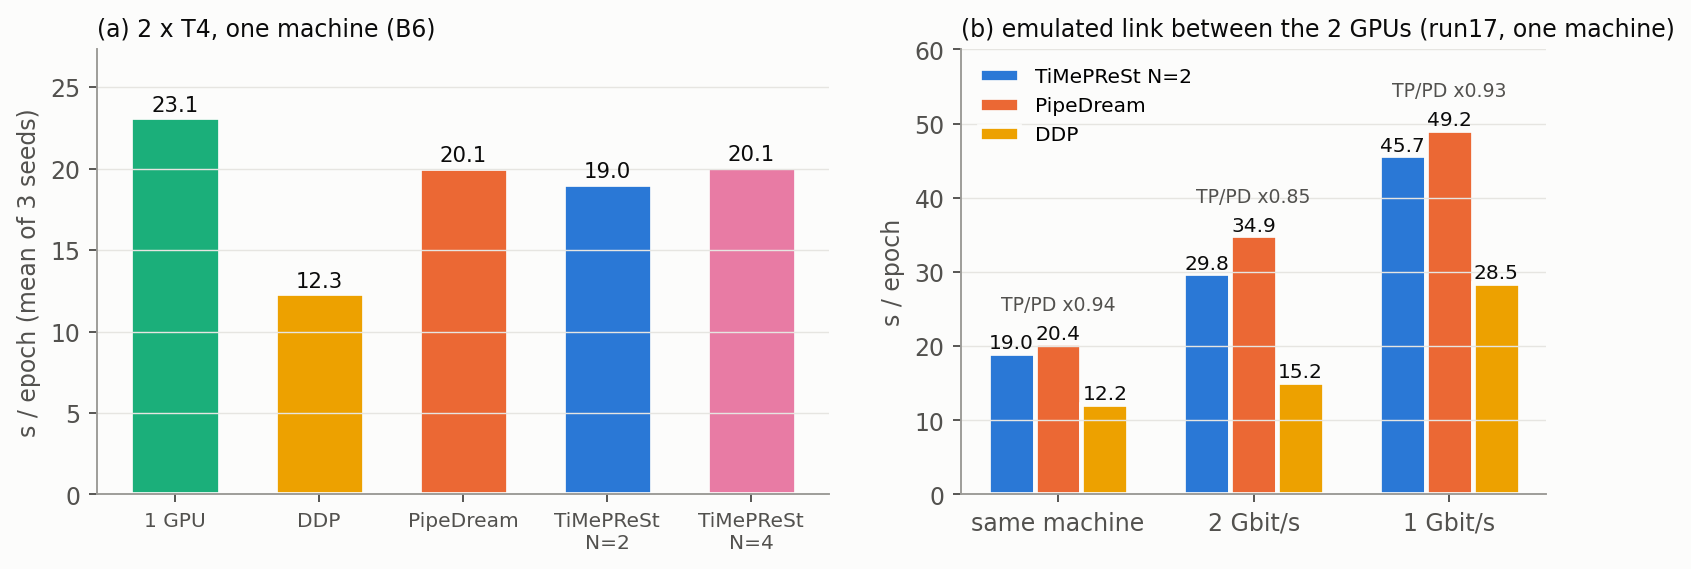
\includegraphics[width=0.84\textwidth]{fig_time.png}
\vspace{0.05cm}
\begin{uitbox}{\faNetworkWired\; Nhận xét}
\scriptsize
Cùng máy, TiMePReSt nhanh hơn PipeDream 5\%; khi giả lập đường truyền 2 / 1 Gbit/s giữa 2 GPU, lợi thế tăng lên \highlight{7--15\%} (hai lần đo, run6 và run17). Nhưng \highlight{DDP vẫn nhanh hơn TiMePReSt 1,6--2,0 lần} ở mọi băng thông: lượng truyền gần bằng nhau (3,2 so với 3,4 GB/epoch), và DDP che khoảng 79\% thời gian truyền vào backward (2 Gbit/s), còn pipeline gần như không che được.
\end{uitbox}
\end{frame}

%--- MAE theo epoch và thời gian ---
\begin{frame}{Sai số theo epoch và tại cùng mốc thời gian}
\centering
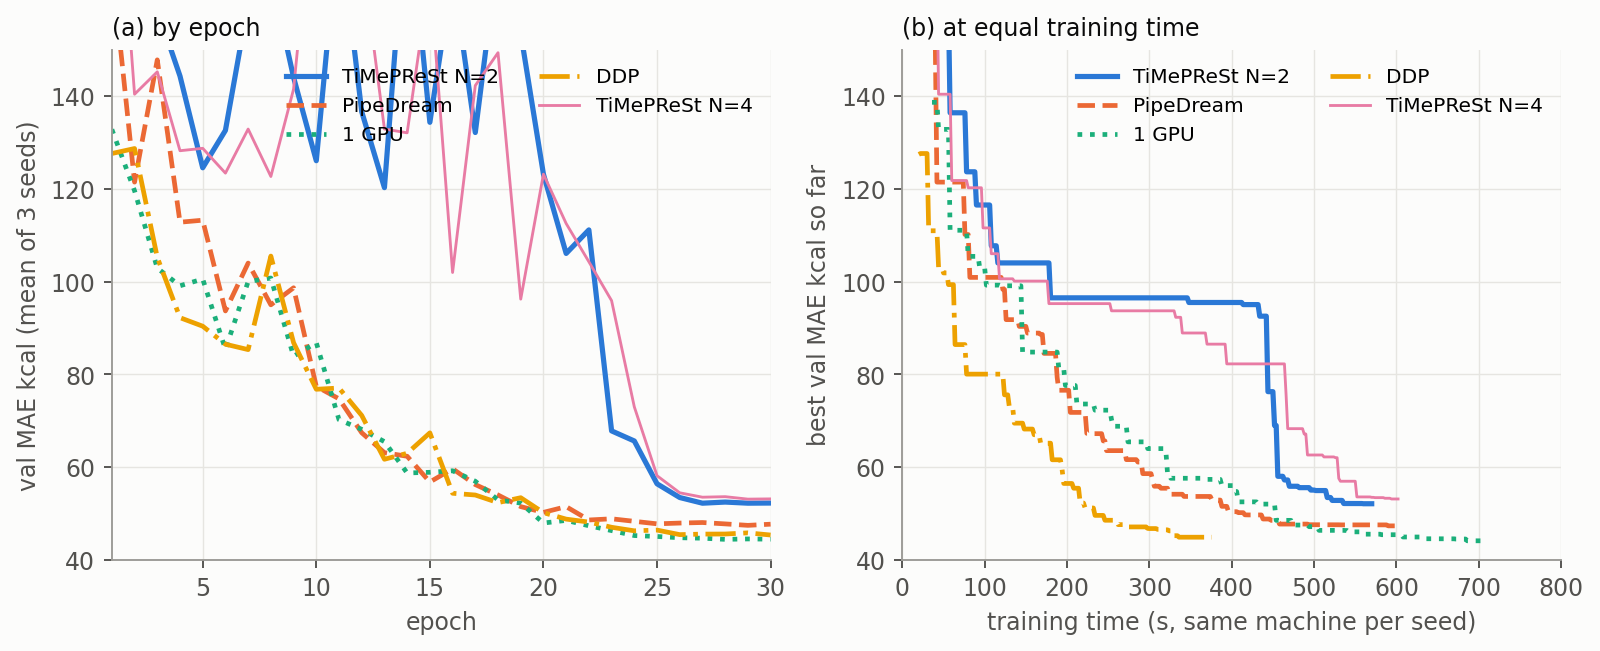
\includegraphics[width=0.78\textwidth]{fig_mae_epoch_time.png}
\vspace{0.05cm}
\begin{uitbox}{\faChartLine\; Nhận xét (val, trung bình 3 seed)}
\scriptsize
Với $w_\text{total} = 3$, TiMePReSt \highlight{kém PipeDream tại mọi mốc thời gian}, kể cả ở đầu (epoch 5: 125 so với 113 kcal; với $w_\text{total} = 1$ nó chỉ nhanh hơn ở đầu). DDP tốt nhất tại mọi mốc: đạt $\le$ 60 kcal sau 193 s, PipeDream 292 s, 1 GPU 321 s, TiMePReSt 455 s.
\end{uitbox}
\end{frame}

%--- Dao động ---
\begin{frame}{Phát hiện: TiMePReSt dao động mạnh ở giữa quá trình}
\centering
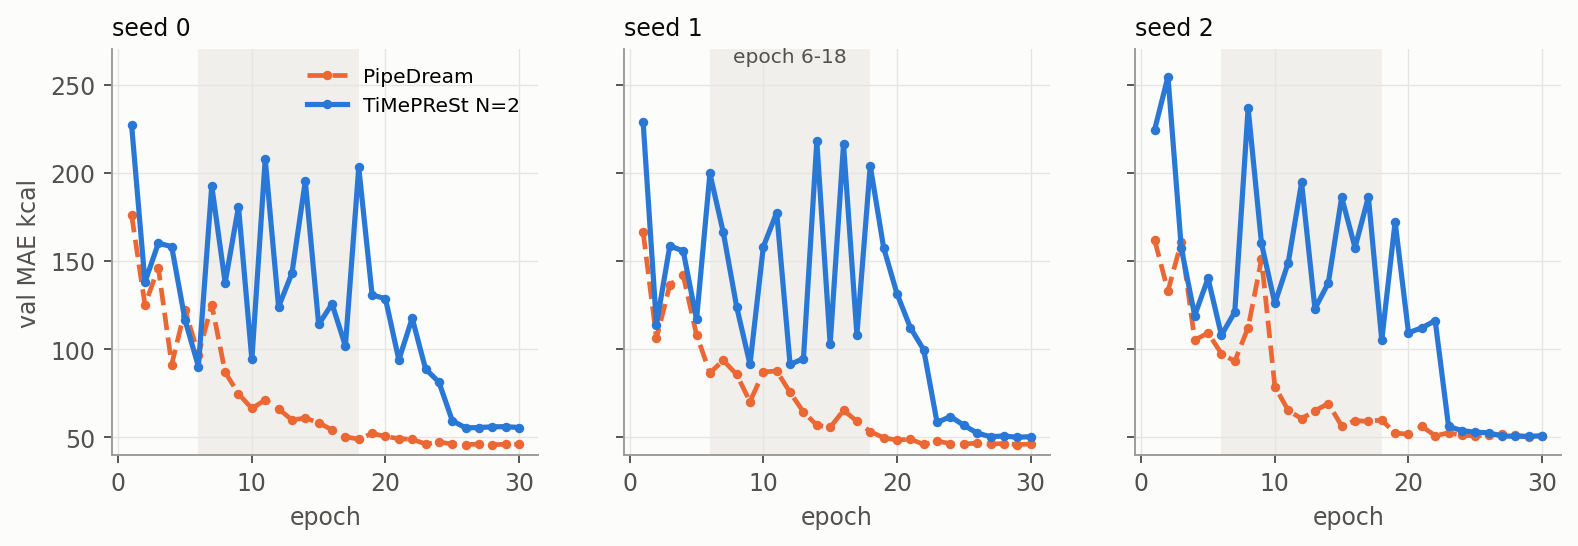
\includegraphics[width=0.80\textwidth]{fig_oscillation.png}
\vspace{0.05cm}
\begin{columns}[T]
\column{0.5\textwidth}
\begin{accentbox}{\faWaveSquare\; Quan sát (cả 3 seed)}
\scriptsize
Epoch 6--18 (lr còn lớn), val MAE của TiMePReSt nhảy kiểu 94 $\rightarrow$ 208, 121 $\rightarrow$ 237 (bước tăng lớn nhất trung bình 117 kcal; PipeDream 28). Hết dao động khi lr giảm. Cuối quá trình TiMePReSt vẫn \kw{underfit}: train MAE 38 so với 27 của PipeDream.
\end{accentbox}
\column{0.44\textwidth}
\begin{uitbox}{\faSearch\; Sweep lr 30 epoch ($w_\text{total} = 1$)}
\scriptsize
Dao động \textbf{không mất} ở lr nào: bước tăng lớn nhất ở epoch 6--18 của TiMePReSt 40--60 kcal (lr 0.005--0.02), PipeDream 8--10 kcal. $\Rightarrow$ do cơ chế (backward dùng trọng số mới hơn lúc forward), không do lr.
\end{uitbox}
\end{columns}
\end{frame}

%--- Sweep lr (tự hiện khi có hình) ---
\IfFileExists{figures/fig_lr_sweep.png}{
\begin{frame}{Sweep lr ở 30 epoch (TiMePReSt và PipeDream, $w_\text{total} = 1$)}
\centering
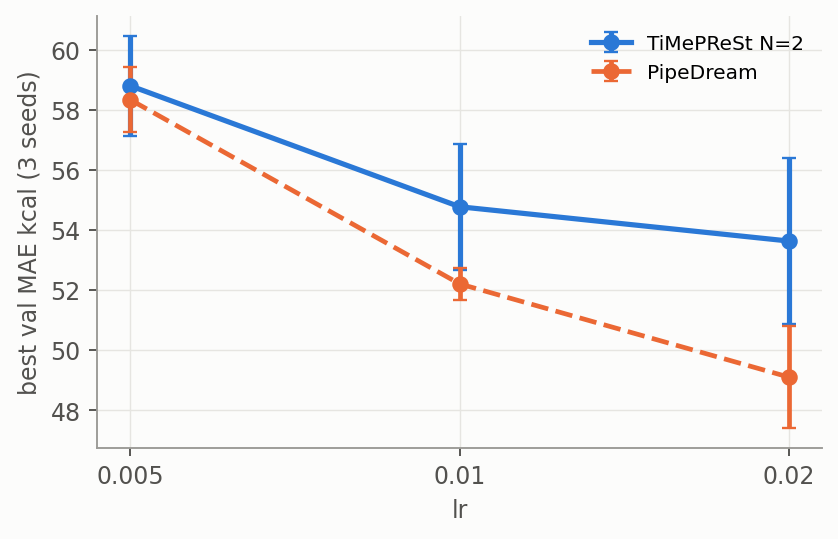
\includegraphics[width=0.55\textwidth]{fig_lr_sweep.png}
\vspace{0.05cm}
\begin{uitbox}{\faSlidersH\; Nhận xét (3 seed mỗi điểm)}
\scriptsize
Cả hai hệ tốt nhất ở lr 0.02. Ở lr tốt nhất, TiMePReSt vẫn kém PipeDream: test 54,7 so với 52,0 kcal (5\%), val 53,6 so với 49,1. lr chỉ giải thích khoảng 1,6 kcal của khoảng cách 8\% ở B6. lr nhỏ hơn làm cả hai hệ kém đi.
\end{uitbox}
\end{frame}
}{}

%--- 60 epoch ---
\begin{frame}{Lịch 60 epoch (trung bình 3 seed, $w_\text{total} = 1$)}
\centering
\scriptsize
\setlength{\tabcolsep}{5pt}
\renewcommand{\arraystretch}{1.2}
\begin{tabular}{@{}llrrrrr@{}}
\toprule
\textbf{Hệ} & \textbf{lr} & \textbf{Epoch} & \textbf{Best val kcal} & \textbf{Test kcal} & \textbf{Test mAP} & \textbf{Tổng thời gian} \\
\midrule
TiMePReSt & 0.01 & 30 / \textbf{60} & 54,8 / 50,7 & 56,3 / \textbf{53,3} & 85,3 / 87,7 & 566 / 1150 s \\
TiMePReSt & 0.02 & 30 / \textbf{60} & 53,6 / 49,4 & 54,7 / \textbf{54,7} & 85,5 / 86,6 & 577 / 1167 s \\
PipeDream & 0.02 & 30 / \textbf{60} & 49,1 / 47,1 & \textbf{52,0} / 53,8 & 86,2 / 87,5 & 596 / 1216 s \\
\bottomrule
\end{tabular}

{\tiny Độ lệch chuẩn test giữa 3 seed: 0,4--1,4 kcal.}

\vspace{0.2cm}
\begin{columns}[T]
\column{0.47\textwidth}
\begin{greenbox}{\faArrowUp\; Thêm epoch}
\scriptsize
\begin{itemize}
  \item Chỉ TiMePReSt lr 0.01 tốt hơn (test $-2{,}9$); lr 0.02 không đổi; PipeDream kém đi $1{,}8$ (train 24,8: overfit).
  \item TiMePReSt (lr chọn theo val: 0.02) \highlight{bắt kịp PipeDream 60 epoch}: kém 0,9 kcal ($<2$).
\end{itemize}
\end{greenbox}
\column{0.47\textwidth}
\begin{accentbox}{\faClock\; Nhưng tính theo tổng thời gian}
\scriptsize
\begin{itemize}
  \item \highlight{PipeDream 30 epoch vẫn tốt nhất} (52,0 trong khoảng 600 s); không cấu hình TiMePReSt nào đạt, kể cả gấp đôi thời gian.
  \item TiMePReSt chỉ nhanh hơn 4--5\%/epoch; dao động 69--84 kcal so với 8.
\end{itemize}
\end{accentbox}
\end{columns}
\end{frame}

%--- Đối chiếu dự đoán ---
\begin{frame}{Đối chiếu với dự đoán ghi trước khi chạy}
\centering
\scriptsize
\setlength{\tabcolsep}{4pt}
\renewcommand{\arraystretch}{1.35}
\begin{tabular}{@{}L{6.2cm}L{6.4cm}@{}}
\toprule
\textbf{Dự đoán (ghi trước, dựa trên phần tái hiện TiMePReSt)} & \textbf{Kết quả trên Nutrition5k} \\
\midrule
MAE cuối TiMePReSt $\approx$ PipeDream & \textcolor{red!60!black}{\textbf{Sai:}} kém 8\% (54,3 so với 50,3) \\
TiMePReSt học nhanh hơn ở giữa quá trình & \textcolor{red!60!black}{\textbf{Sai:}} kém ở mọi mốc, dao động mạnh ($w_\text{total} = 1$: chỉ đúng ở epoch $\le$ 5) \\
Cùng máy: DDP nhanh nhất; TiMePReSt có thể chậm hơn PipeDream & \textcolor{greenteal}{\textbf{Đúng phần DDP;}} TiMePReSt lại nhanh hơn PipeDream 5\% \\
Mạng 1--2 Gbit/s: TiMePReSt nhanh hơn PipeDream & \textcolor{greenteal}{\textbf{Đúng:}} nhanh hơn 7--15\% (nhưng DDP vẫn nhanh hơn) \\
Bộ nhớ TiMePReSt và PipeDream gần như nhau & \textcolor{greenteal}{\textbf{Đúng:}} 8283 so với 8360 MB ở GPU0 \\
\bottomrule
\end{tabular}
\end{frame}

\section{Bản đồ calories}

%--- Ví dụ bản đồ ---
\begin{frame}{Bản đồ calories và CAM của từng nguyên liệu (TiMePReSt)}
\centering
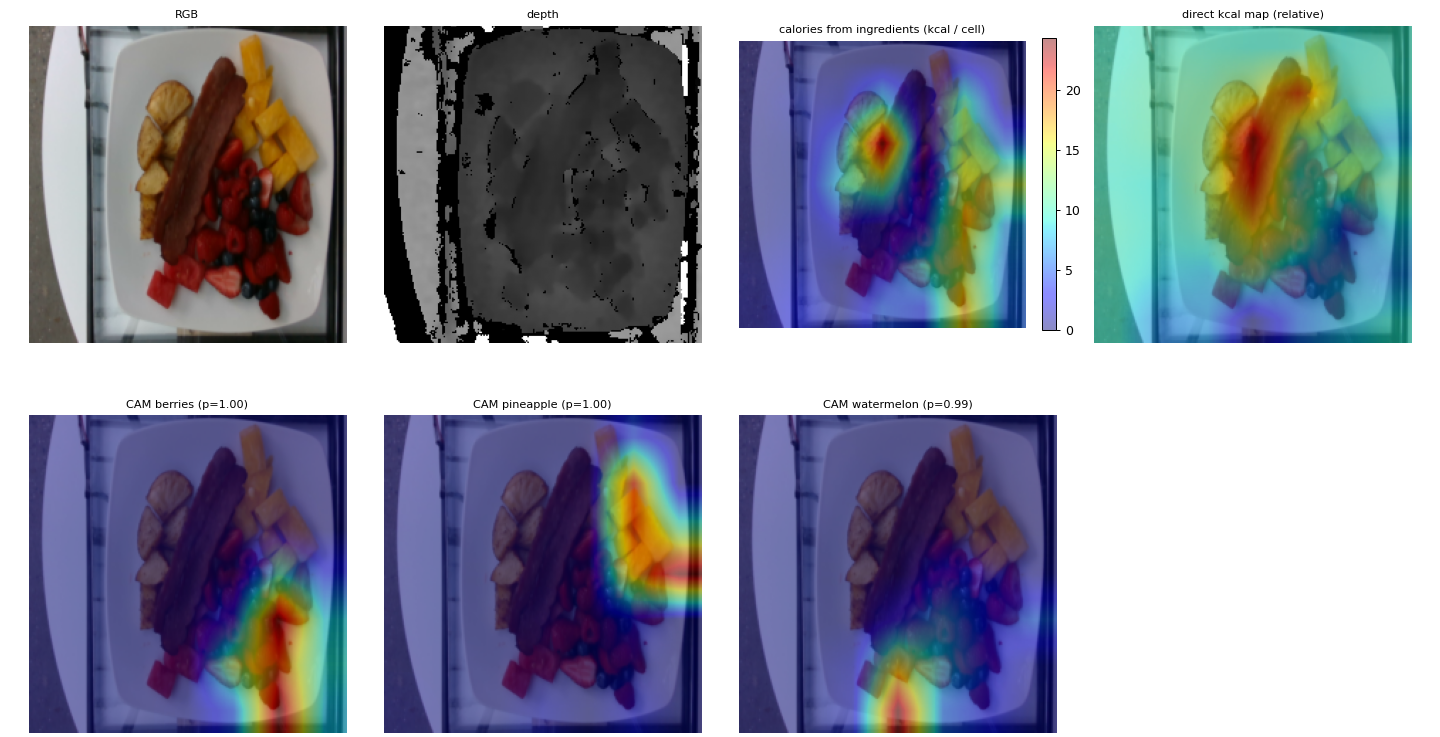
\includegraphics[width=0.66\textwidth]{fig_map_1562170356.png}
\vspace{0.02cm}
\begin{uitbox}{\faMap\; Cách tính}
\scriptsize
Với nguyên liệu $k$ đoán có ($p \ge 0{,}5$): $A_k = \mathrm{ReLU}(\mathrm{CAM}_k) / \sum \mathrm{ReLU}(\mathrm{CAM}_k)$; bản đồ calories $C = \sum_k \mathrm{kcal}_k \cdot A_k$ (tổng bằng kcal của các nguyên liệu đoán có). Món này: thật 385 kcal, đoán 301 kcal.
\end{uitbox}
\end{frame}

%--- Deletion test ---
\begin{frame}{Bản đồ có trung thực với mô hình không? (deletion test)}
\begin{columns}[T]
\column{0.58\textwidth}
\centering
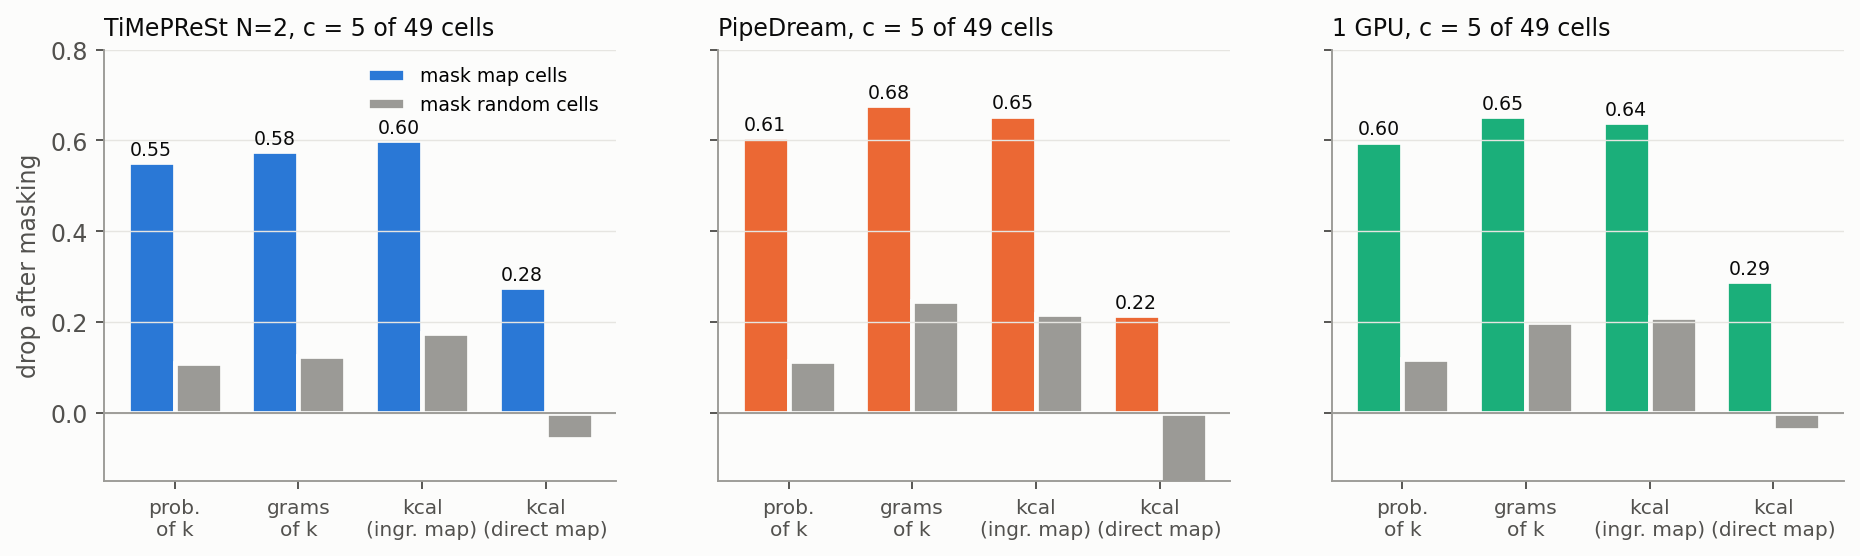
\includegraphics[width=\textwidth]{fig_deletion.png}

\vspace{0.1cm}
\scriptsize
Che 5 / 49 ô (lưới 7$\times$7) có giá trị cao nhất của bản đồ, so với che 5 ô ngẫu nhiên; 486 món test, khoảng 3000 cặp (món, nguyên liệu).
\column{0.39\textwidth}
\begin{greenbox}{\faCheck\; Theo quy tắc ghi trước}
\scriptsize
Cả 4 loại bản đồ đều \highlight{trung thực với mô hình}, ở cả TiMePReSt, PipeDream và 1 GPU (Wilcoxon $p < 10^{-76}$; che theo bản đồ giảm nhiều hơn ở 93--97\% trường hợp).
\end{greenbox}
\vspace{0.1cm}
\begin{accentbox}{\faExclamationTriangle\; Giới hạn}
\scriptsize
\begin{itemize}
  \item CAM chỉ riêng \kw{một phần} cho từng nguyên liệu: che CAM của $k$ cũng làm nguyên liệu khác giảm 0,33--0,38 (ngẫu nhiên 0,14).
  \item Bản đồ calories cho \kw{phân bố}, không cho con số chính xác (tổng $\approx$ 0,7 lần kcal trực tiếp).
  \item Deletion test chỉ cho "trung thực với mô hình"; vị trí thật đo ở slide sau bằng mask.
\end{itemize}
\end{accentbox}
\end{columns}
\end{frame}

%--- Vị trí so với mask thật ---
\begin{frame}{Bản đồ có đúng vị trí thật không? (mask nguyên liệu HandMasks)}
\centering
\scriptsize
\setlength{\tabcolsep}{5pt}
\renewcommand{\arraystretch}{1.2}
\begin{tabular}{@{}lrrr@{}}
\toprule
\textbf{Hệ} (bản đồ calories) & \textbf{M1: kcal trên thức ăn} & \textbf{M2: sai số tỉ lệ kcal vùng} & \textbf{M3: pointing} \\
\midrule
Mốc (đều / diện tích / ngẫu nhiên) & 0,18 & 0,190 & 0,50 \\
1 GPU & \textbf{0,52} & 0,159 ($-16\%$) & 0,85 \\
PipeDream & \textbf{0,52} & \textbf{0,147} ($-22\%$) & 0,83 \\
TiMePReSt & 0,51 & 0,151 ($-21\%$) & \textbf{0,85} \\
\bottomrule
\end{tabular}

\vspace{0.15cm}
\begin{columns}[T]
\column{0.5\textwidth}
\begin{uitbox}{\faMap\; Dữ liệu và cách đo}
\scriptsize
Mask nguyên liệu do Hand và cộng sự vẽ trên chính ảnh Nutrition5k \cite{hand2026segmentation}: 154 món test của mình (mô hình chưa thấy), mỗi vùng có kcal thật. So ở lưới 7$\times$7 của bản đồ. Quy tắc ghi trước; Wilcoxon $p < 0{,}01$.
\end{uitbox}
\column{0.44\textwidth}
\begin{greenbox}{\faCheck\; Kết quả}
\scriptsize
Cả 3 hệ đạt cả 3 metric: bản đồ \highlight{đặt kcal lên đúng vùng thức ăn thật} và chia kcal giữa các vùng đúng hơn chia theo diện tích. Giới hạn: chỉ khoảng một nửa kcal nằm trên thức ăn (lưới thô); hành, tỏi gần mức ngẫu nhiên.
\end{greenbox}
\end{columns}
\end{frame}

\section{Thí nghiệm phụ và so sánh}

%--- Two-stream ---
\begin{frame}{Thí nghiệm phụ: mô hình two-stream (ResNet-50 RGB + ResNet-50 depth)}
\begin{columns}[T]
\column{0.48\textwidth}
\begin{uitbox}{\faImages\; Chất lượng (1 GPU, 8 epoch, 2 seed)}
\scriptsize
\setlength{\tabcolsep}{4pt}
\begin{tabular}{@{}lrr@{}}
\toprule
 & \textbf{Một nhánh} & \textbf{Two-stream} \\
\midrule
Val MAE kcal & 64,9 & \textbf{62,2} \\
Val mAP & 70,2 & \textbf{73,8} \\
Test MAE kcal & 64,1 & \textbf{59,1} \\
s/epoch & 27,5 & 59,2 (2,15$\times$) \\
Peak GPU & 5,6 GB & 13,8 GB \\
\bottomrule
\end{tabular}
\end{uitbox}

\column{0.48\textwidth}
\begin{accentbox}{\faServer\; Trên 2 GPU (cùng máy, 8 epoch)}
\scriptsize
\begin{itemize}
  \item Chỉ cách chia \texttt{[0,4,18]} vừa bộ nhớ: GPU0 phải giữ activation của 2 mini-batch.
  \item So với 1 GPU: DDP \highlight{0,51$\times$} thời gian; PipeDream 1,12$\times$; TiMePReSt 1,10$\times$ (pipeline \textbf{chậm hơn} 1 GPU).
  \item TiMePReSt / PipeDream = 0,986; TiMePReSt kém 13\% kcal.
\end{itemize}
\end{accentbox}
\vspace{0.1cm}
\begin{greenbox}{\faFlag\; Quyết định}
\scriptsize
Giữ mô hình một nhánh làm kết quả chính. Two-stream là ví dụ: mô hình nặng hơn nhưng vẫn vừa 1 GPU thì pipeline bất đồng bộ không có lợi.
\end{greenbox}
\end{columns}
\end{frame}

%--- So sánh tài liệu ---
\begin{frame}{So sánh với các nghiên cứu khác trên Nutrition5k}
\begin{columns}[T]
\column{0.56\textwidth}
\begin{uitbox}{\faBook\; Sai số calo (\% so với giá trị trung bình)}
\scriptsize
\setlength{\tabcolsep}{4pt}
\begin{tabular}{@{}L{3.6cm}L{1.6cm}r@{}}
\toprule
\textbf{Công trình} & \textbf{Đầu vào} & \textbf{Sai số} \\
\midrule
Nutrition5k (2021), trực tiếp & RGB & 26,1\% \\
Nutrition5k, depth làm kênh 4 & RGB-D & 18,8\% \\
Nutrition5k, ước thể tích & RGB-D & 16,5\% \\
\textbf{Của em: 1 GPU / PipeDream} & RGB-D & \textbf{19,5\%} \\
\textbf{Của em: TiMePReSt} & RGB-D & 21,1\% \\
DPF-Nutrition (2023) & RGB + depth dự đoán & 14,7\% \\
RDINet (2026) & RGB-D & 14,9\% \\
IGSMNet (2025) & RGB-D + ngữ nghĩa & 12,2\% \\
\bottomrule
\end{tabular}
\end{uitbox}
\column{0.40\textwidth}
\begin{accentbox}{\faInfoCircle\; Nhận xét}
\scriptsize
\begin{itemize}
  \item Ngang cách tương ứng của bài gốc (depth làm kênh thứ 4).
  \item Kém các bài mới 5--7 điểm \%: các bài đó tách hai nhánh RGB / depth, có module hợp nhất.
  \item Không so tuyệt đối được: mỗi bài chia train/test khác nhau; số liệu do các bài tự báo cáo.
  \item Trọng tâm của em là \kw{hệ thống huấn luyện}, không phải mô hình dinh dưỡng tốt nhất.
\end{itemize}
\end{accentbox}
\end{columns}
\end{frame}

\section{Kết luận}

%--- Kết luận ---
\begin{frame}{Kết luận, hạn chế và việc tiếp theo}
\begin{columns}[T]
\column{0.5\textwidth}
\begin{uitbox}{\faFlag\; Kết luận}
\scriptsize
\begin{itemize}
  \item TiMePReSt chạy đúng trên bài toán hồi quy đa nhiệm (kiểm tra PASS), nhanh hơn PipeDream 5\% (7--15\% khi mạng chậm), nhưng \highlight{kém 8\% MAE} (30 epoch) và dao động mạnh giữa quá trình; 60 epoch thì bắt kịp PipeDream 60 epoch nhưng \highlight{không đạt PipeDream 30 epoch}.
  \item Trên 2 GPU, \highlight{DDP tốt nhất} ở mọi tiêu chí, cả khi mạng chậm.
  \item Bản đồ calories \highlight{trung thực} và \highlight{đúng vị trí thật} hơn rõ so với mốc (mask), cả với TiMePReSt.
\end{itemize}
\end{uitbox}
\vspace{0.1cm}
\begin{accentbox}{\faExclamationTriangle\; Hạn chế}
\scriptsize
Chỉ $W = 2$ GPU, một loại phần cứng, một dataset; mô hình vừa 1 GPU; sweep lr và 60 epoch mới có ở một số cấu hình; chọn theo val trên 486 món có nhiễu 1--2 kcal.
\end{accentbox}

\column{0.46\textwidth}
\begin{greenbox}{\faTasks\; Đang chạy / đề xuất}
\scriptsize
\begin{itemize}
  \item \kw{Đã xong:} sweep lr 30 epoch và bản đồ calories cho cả TiMePReSt và PipeDream (để chọn một trong hai làm phương pháp chính).
  \item \kw{Đã xong:} lịch 60 epoch (3 seed): PipeDream 30 epoch vẫn tốt nhất.
  \item \kw{Đã xong:} DDP khi mạng chậm: vẫn nhanh hơn TiMePReSt 1,6--2,0 lần ở 2 / 1 Gbit/s.
\end{itemize}
\end{greenbox}
\vspace{0.1cm}
\begin{uitbox}{\faQuestionCircle\; Xin ý kiến anh}
\scriptsize
\begin{itemize}
  \item Vị trí thật đã đo bằng mask HandMasks (cùng ảnh Nutrition5k); như vậy đã đủ chưa, hay cần thêm một dataset khác?
  \item Kết quả hiện tại nên viết thành bài theo hướng "khi nào TiMePReSt có lợi" không, và gửi ở đâu?
\end{itemize}
\end{uitbox}
\end{columns}
\end{frame}

%--- Tài liệu tham khảo ---
\begin{frame}[allowframebreaks]{Tài liệu tham khảo}
\tiny
\nocite{dpfnutrition,rdinet,igsmnet}
\bibliographystyle{apalike}
\bibliography{references}
\end{frame}

\end{document}
